\section{Response to Reviewer 16}
\begin{bibunit}[alpha]
\textbf{Reviewer 16---General comments---}\textit{%
This paper addresses linear control over wireless links with imperfect channel-state information, formulating a hidden Markov jump linear system that transmits multiple future inputs with dropout compensation.
Its contributions include both finite and infinite-horizon LQR solutions and a spectral-radius-based stability condition. The manuscript is concise and well-structured. There are some comments and questions that the authors are invited to consider.}\\[2mm]
\textbf{Authors' response:} \textcolor{black}{We sincerely appreciate the Reviewer's careful reading of our paper and their valuable comments. We have addressed each of them below.}\\[4mm]
%%%
\textbf{Reviewer 16---Comment 1---}\textit{%
You introduce a parameter $L$ (the maximal number of consecutive control message dropouts) and show that for large enough dropout intervals, certain transition probabilities become negligible. 
In practice, is $L$ purely a theoretical bound, or is it also enforced by additional network constraints (e.g., maximum re-transmissions)?}\\[2mm]
\textbf{Authors' response to comment 1:} \textcolor{black}{We thank the Reviewer for the valuable comment. 
The maximal number of consecutive control message dropouts, $L$, is an intrinsic characteristic of the finite-state Markov channel (FSMC), the detector observing it, and the model reliability threshold, $\epsilon$. We use the machine epsilon as the threshold $\epsilon$ to obtain the most reliable numerical results. The emission probability matrix, $P_e$, indicates the quality of the practical channel state information (CSI), ranging from perfect CSI, which is often challenging to obtain, to no CSI. This letter follows the analytical framework from [12] to rely on the FSMC characterization at the message or packet level, meaning that the successful delivery probability (SDP) accounts for all relevant communication constraints, comprising signal-processing and diversity techniques. This includes, for instance, path diversity, channel encoding, multiple antennas, and re-transmissions. Consequently, $L$ accounts for all practical communication constraints of an FSMC that operates with the control application timing. Please refer to [12] for additional details on the FSMCs for wireless networked control systems coupled design.}\\[4mm]
%%%
\textbf{Reviewer 16---Comment 2---}\textit{%
The ergodicity assumption (A.4) ensures the existence of a steady-state probability $\pi(\infty)$ for the channel. 
Are there scenarios where $\{\theta_k\}$ is non-ergodic (e.g., absorbing states or block-fading channels)? 
How would your results be modified or extended to handle a partially ergodic or slowly time-varying model?}\\[2mm]
\textbf{Authors' response to comment 2:} \textcolor{black}{We are thankful to the Reviewer for a thoughtful comment. The ergodicity assumption (A.4) is used only in the infinite-horizon setting, addressed in Sections VI–VIII. The finite-horizon results are directly applicable to the time-varying setting if the underlying time-varying FSMC model is known. If the FSMC model is polytopic time-inhomogeneous (PTI)—that is, its transition probability matrices (TPMs) and SDP vectors are time-varying within a known polytopic set, and their exact values are unknown—the results of this letter could be extended by following the ideas of \cite{zacchialun2025lcss}. Regarding the infinite-horizon setting without the ergodicity assumption, we must distinguish between the non-ergodic and slowly time-varying cases. To our knowledge, all realistic FSMCs that operate with the control application timing are ergodic. These models incorporate block fading and do not admit absorbing states. So, we do not delve into non-ergodic settings, but we would be interested in learning about time-homogeneous non-ergodic FSMCs of practical relevance. Regarding the slowly time-varying case, our infinite-horizon analysis can be helpful if the channel variations are slower than the closed-loop system transient. If less than one, the spectral radius of the mean-square stability verification matrix, $\rho(\mathit{\Lambda})$, indicates exponential convergence rate, as detailed in our response to the Reviewer’s next question.}\\[4mm]
%%%
\textbf{Reviewer 16---Comment 3---}\textit{%
In Theorem 4, $\rho(\Lambda) < 1$ is the condition for mean-square stability. 
Beyond guaranteeing $\rho(\Lambda) < 1$, do you have insights on how quickly the states converge in practice? 
Is there a known rate of convergence or mixing time for the underlying Markov chain that
influences closed-loop transient behaviour?}\\[2mm]
\textbf{Authors' response to comment 3:} \textcolor{black}{We are grateful to the Reviewer for an excellent question. The condition $\rho(\Lambda)<1$ is necessary and sufficient for the mean-square stability (MSS) of a (hidden) Markov jump linear system (MJLS). According to the MJLS theory presented in \cite{costa2006discrete} and \cite{zacchialun2019automatica}, MSS is equivalent to exponential MSS even in the PTI setting, and the value of the (joint) spectral radius of the mean-square stability verification matrix relates to the maximal exponential decay rate. Please refer to the proofs of \cite[Prop. 3.25]{costa2006discrete} and \cite[Thm. 14, 16]{zacchialun2019automatica} for additional technical details.}\\[4mm]
%%%
\textbf{Reviewer 16---Comment 4---}\textit{%
In many industrial or mobile scenarios, channel statistics can drift over time (e.g., changes in multipath profiles, device mobility). 
Does your framework allow for slowly time-varying TPMs $P_c$ or detection matrices $P_e$?}\\[2mm]
\textbf{Authors' response to comment 4:} \textcolor{black}{We thank the Reviewer for the relevant question. As detailed in our responses to the Reviewer's previous questions, our framework allows for time-varying TPMs and SDP vectors. If TPM and SDP values are known, our finite-horizon results can be applied directly. Similar to \cite{zacchialun2025lcss}, if TPMs and SDP vectors are unknown but bounded by the known polytopic sets, the finite-horizon results could be extended to account for such a setting. The infinite-horizon theoretical results could be extended to the PTI setting via \cite{zacchialun2019automatica} and \cite{zacchialun2019ecc}, but computing the joint spectral radius over a set of relevant mean-square stability verification matrices may be currently computationally unfeasible—please see our response to the Reviewer's fifth comment for additional details. 
Finally, the infinite-horizon results presented in this letter can be applied to settings with slowly varying TPMs and SDP vectors, as long as their values are known and channel variations happen more slowly than the transients of the closed-loop system. To this end, this letter demonstrates that a careful choice of the number of future control inputs included in the controller's messages, along with the message dropout compensation strategy, can significantly reduce the value of $\rho(\Lambda)$ and shorten the transient phase of the closed-loop system. Regarding the emission probability matrices $P_e$, we would leave them constant since they represent the practical constraints of a detector and account for the general quality of available CSI. In other words, $P_e$ is a parameter of the CSI detection schemes and can be used as a wireless networked control system design parameter.}\\[4mm]
%%%
\textbf{Reviewer 16---Comment 5---}\textit{%
Could you comment on how the computational burden scales with $N$, $M$, and $n_f$? 
For instance, how feasible is the approach for larger state spaces or multiple clusters?}\\[2mm]
\textbf{Authors' response to comment 5:} \textcolor{black}{We thank the Reviewer for an excellent question. The number of discrete states of the hidden MJLS mainly determines the computational burden. This discrete state space is given by the product of $L+1$ and $M$ or $M^2$, as indicated by (25) and (42). $L$ increases with the message error rate of the FSMC and with lower model reliability thresholds $\epsilon$. For instance, this letter's numerical example considers an FSMC with a high average message dropout probability (AMDP) of 9.075\% and $\epsilon = 2.220446049250313\cdot 10^{-16}$. This setting results in $L = 27$. Setting  $\epsilon = 10^{-12}$ would lead to $L = 20$, thus reducing complexity and model reliability. $M\leq N$. Designing a controller with fewer detector states reduces the computational burden at the expense of increased control cost, as shown in Fig. \ref{fig:stability-coeff-16}, reproduced below, for the Reviewer's convenience.
\setcounter{figure}{2}
\begin{figure}[h!]
\begin{center}
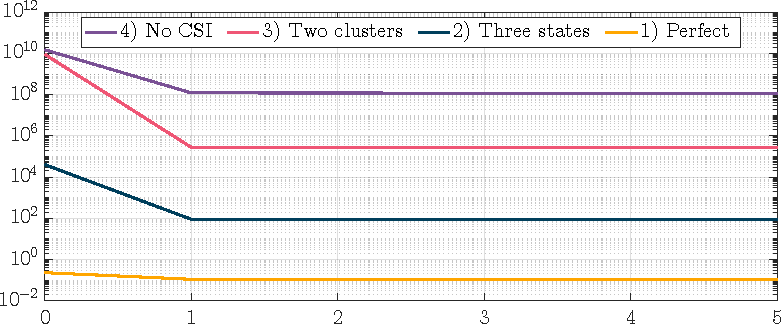
\includegraphics[width=0.76\columnwidth]{cost-cntrl-a.pdf}
%\includegraphics[width=0.7\columnwidth]{./responses-rev-1/stability-cntrl-2.pdf}
\caption{The long-run average cost $J_{\infty}^{\star}$ from (50b) as a function of $n_f$.}\label{fig:stability-coeff-16}
\end{center}
\end{figure}\\
The no-CSI setting incurs the lowest computational burden, while the perfect CSI setting is the most computationally demanding. Finding an optimal infinite-horizon controller in the mode-independent (no-CSI, $M=1$) setting has a low computational burden for any given FSMC, regardless of the number of its states $N$, if $L$ is the same. This makes the mode-independent control strategy particularly appealing for scenarios with many discrete and continuous states (i.e., $N$ and $n_x$ big). Finally, $n_f+1$ is a multiplicative factor that determines the number of control inputs. It only affects the number of basic matrix operations required by (11), (13), (22), (23), and their combination in (24), which has a limited impact on overall complexity. Unfortunately, because of the strict page limit of an L-CSS letter, we could not include any of these insights in the revised version of the manuscript.}\\[4mm]
%%%
\textbf{Reviewer 16---Comment 6---}\textit{%
Does having $\Phi\neq I$, ever risk a slow return to equilibrium if the dropout period is large, or is it primarily beneficial to prevent states from diverging in the short term?}\\[2mm]
\textbf{Authors' response to comment 6:} \textcolor{black}{We thank the Reviewer for a pertinent question. As detailed in the response to Reviewer 9's second question on parameter tuning, for the linearized model of a rotary inverted pendulum considered in this letter, $\mathit{\Phi}=I$ yields the highest values of $\rho(\mathit{\Lambda})$ and $J_{\infty}^{\star}$, resulting in the poorest performance in terms of control cost and transient length. For the Reviewer's convenience, we show the relevant figures below.
%%
\setcounter{figure}{0}
\begin{figure}[h!]
\begin{center}
\includegraphics[width=0.7\columnwidth]{stability-cntrl-2.pdf}
\caption{The spectral radius of the mean-square stability verification matrix, $\rho(\mathit{\Lambda})$, as a function of the dropout compensation factor $\mathit{\Phi}$ for the rotary inverted pendulum under the proposed infinite-horizon linear–quadratic regulation (LQR) with $n_f=0$ [4—Fig. 12]}
\end{center}
\end{figure}
\vspace*{-10pt}
\begin{figure}[h!]
\begin{center}
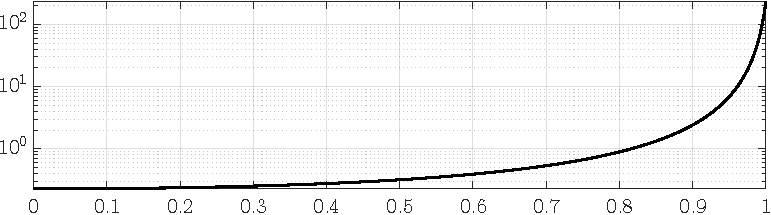
\includegraphics[width=0.7\columnwidth]{cost-cntrl-2.pdf}
\caption{Long-run average cost $J_{\infty}^{\star}(\mathit{\Phi})$ for the rotary inverted pendulum under the proposed infinite-horizon LQR with $n_f=0$ for $\Sigma_{w}=4\cdot 10^{-6} I_4$. See [4—Fig. 13] for similar results, obtained with $\Sigma_{w}=2.5\cdot 10^{-9} I_4$.}
\end{center}
\end{figure}
\vspace*{-10pt}
\setcounter{figure}{3}
\begin{figure}[h!]
\begin{center}
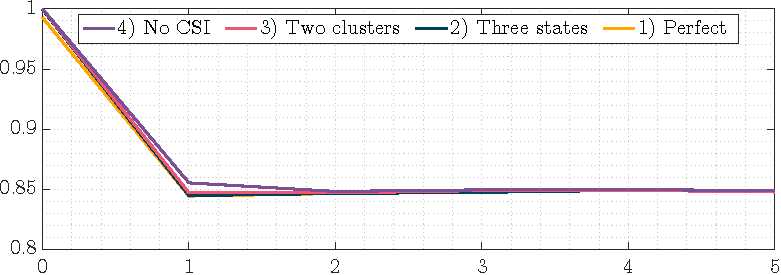
\includegraphics[width=0.7\columnwidth]{stability-cntrl-1.pdf}
\caption{The spectral radius of the mean-square stability verification matrix, $\rho(\mathit{\Lambda})$, as a function of the number of control inputs $n_f$ for the rotary inverted pendulum under the proposed infinite-horizon linear–quadratic regulation (LQR) with the dropout compensation factor $\mathit{\Phi}=I$}
\end{center}
\end{figure}
% \vspace*{10pt}
\begin{figure}[h!]
\begin{center}
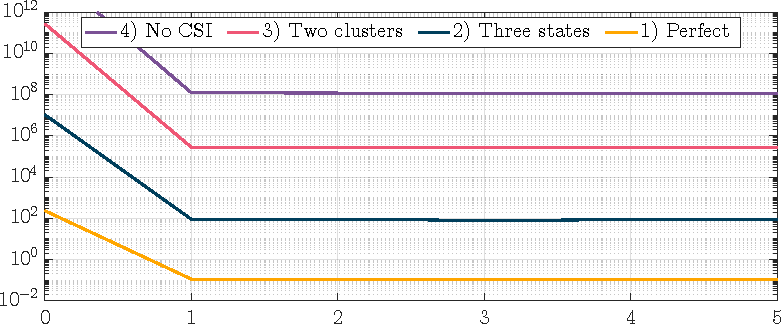
\includegraphics[width=0.7\columnwidth]{cost-cntrl-1.pdf}
\caption{The long-run average cost, $J_{\infty}^{\star}$, as a function of the number of control inputs $n_f$ for the rotary inverted pendulum under the proposed infinite-horizon linear–quadratic regulation (LQR) with the dropout compensation factor $\mathit{\Phi}=I$}
\end{center}
\end{figure}
% \vspace*{10pt}
\begin{figure}[h!]
\begin{center}
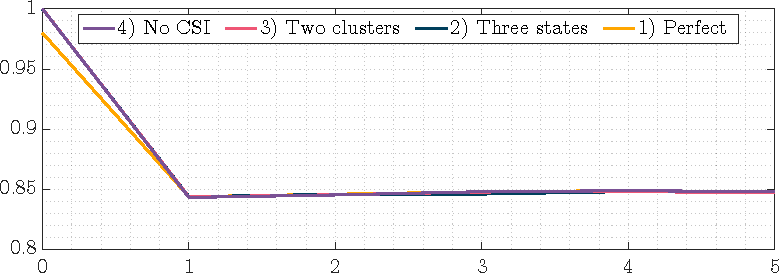
\includegraphics[width=0.76\columnwidth]{stability-cntrl-9.pdf}
\caption{The spectral radius of the mean-square stability verification matrix, $\rho(\mathit{\Lambda})$, as a function of the number of control inputs $n_f$ for the rotary inverted pendulum under the proposed infinite-horizon linear–quadratic regulation (LQR) with the dropout compensation factor $\mathit{\Phi}=0.921$}
\end{center}
\end{figure}
\vspace*{10pt}
\begin{figure}[h!]
\begin{center}
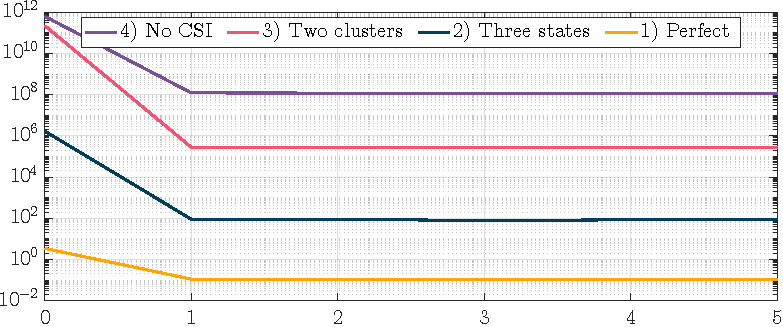
\includegraphics[width=0.76\columnwidth]{cost-cntrl-9.pdf}
\caption{The long-run average cost, $J_{\infty}^{\star}$, as a function of the number of control inputs $n_f$ for the rotary inverted pendulum under the proposed infinite-horizon linear–quadratic regulation (LQR) with the dropout compensation factor $\mathit{\Phi}=0.921$}
\end{center}
\end{figure}\\
\newpage
\begin{figure}[h!]
\begin{center}
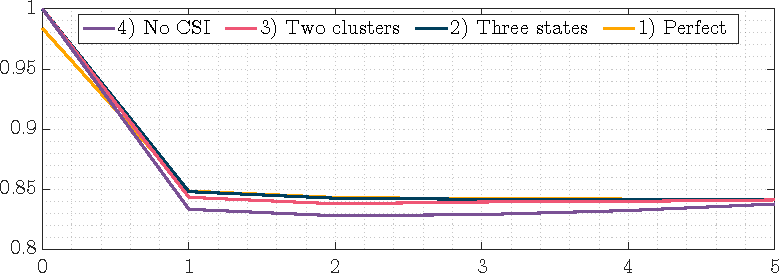
\includegraphics[width=0.76\columnwidth]{stability-cntrl-0.pdf}
\caption{The spectral radius of the mean-square stability verification matrix, $\rho(\mathit{\Lambda})$, as a function of the number of control inputs $n_f$ for the rotary inverted pendulum under the proposed infinite-horizon linear–quadratic regulation (LQR) with the dropout compensation factor $\mathit{\Phi}=0$}
\end{center}
\end{figure}
\begin{figure}[h!]
\begin{center}
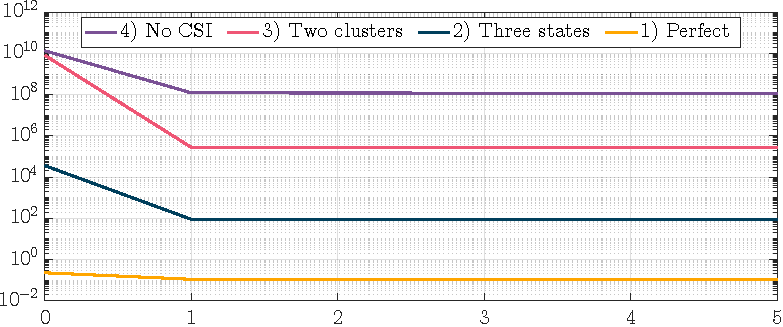
\includegraphics[width=0.76\columnwidth]{cost-cntrl-0.pdf}
\caption{The long-run average cost, $J_{\infty}^{\star}$, as a function of the number of control inputs $n_f$ for the rotary inverted pendulum under the proposed infinite-horizon linear–quadratic regulation (LQR) with the dropout compensation factor $\mathit{\Phi}=0$}
\end{center}
\end{figure}
%%
% As discussed in our response to the Reviewer's third comment, the value of $\rho(\mathit{\Lambda})$ relates to the maximal exponential decay rate.
Please also refer to our response to Reviewer 10's sixth comment on technical accuracy, in which we analyzed the closed-loop system performance under exceptionally high average message dropout probabilities exceeding $21.4$\%, which further increases with the size of the control message due to the growing number of future control inputs.
For the mode-independent scenario (No CSI) with $\mathit{\Phi}=0.1$, transmitting more than three future control inputs may destabilize the closed-loop system due to high message error rate. However, these observations may not apply to different plants and FSMCs. The presented framework allows us to investigate the impact of any specific message dropout strategy $\mathit{\Phi}$ on the transient and steady-state behavior of any linear plant controlled through an FSMC with potentially imperfect CSI.}\\[4mm]
%%%
\textbf{Reviewer 16---Comment 7---}\textit{%
How might the approach adapt to input/state constraints or nonlinear systems?}\\[2mm]
\textbf{Authors' response to comment 7:} \textcolor{black}{We thank the Reviewer for an insightful question. Although we do not yet have a ready extension for constrained and nonlinear systems, we may try to adopt the ideas of \cite{KOTHARE19961361} to incorporate constraints and \cite{10273597} to address nonlinearities.}\\[4mm]
%%%
\textbf{Authors' concluding remark:} \textcolor{black}{We thank the Reviewer for the valuable comments and suggestions. We sincerely hope the above explanations have adequately addressed the Reviewer's concerns.}
\putbib
\end{bibunit}